\documentclass[11pt,UTF8]{beamer}
\usetheme{metropolis}
\metroset{progressbar=frametitle,numbering=fraction}
\usepackage{bm}
\usepackage{amsmath,amssymb,amsfonts}
\usepackage{booktabs}
\usepackage{graphicx}
\usepackage{xcolor}
\usepackage{tikz}
\usetikzlibrary{calc,positioning,decorations.pathmorphing}
\setbeamercolor{block title}{use=normal text, fg=normal text.fg,bg=normal text.bg!80!fg}
\setbeamercolor{mymath}{use={block title, normal text}, bg=block title.bg!50!normal text.bg}
\setbeamercolor{mymath2}{bg=blue!10, fg=black}
\graphicspath{{./figures/}{./logo/}{../draft/figures/prl/}}

%%%%%%%%%%%%% Macros %%%%%%%%%%%%%
\newcommand{\rmi}{\mathrm{i}}
\newcommand{\rmd}{\mathrm{d}}
\newcommand{\blockbodygap}{\vspace{0.3em}}
\newcommand{\afterblockgap}{\vspace{0.45em}}

\title{Generative Modeling of Real-Time\\ Stochastic Dynamics}
\subtitle{}

\date{August 2026}
\author{Yang-yang Tan}
% \institute{The University of Tokyo \& RIKEN iTHEMS}
\titlegraphic{%
  \begin{tikzpicture}[remember picture, overlay]
    % Top-left: school name
    \node[anchor=north west, inner sep=0pt, font=\normalsize\bfseries, text=burgundy]
      at ([xshift=0.6cm,yshift=-0.5cm]current page.north west)
      {AI for Science Summer School};
    % Bottom-right: UTokyo + IPI (aligned with author/date)
    \node[anchor=south east, inner sep=0pt] (utokyo) at ([xshift=-0.6cm,yshift=2.9cm]current page.south east) {%
      \raisebox{-0.5\height}{\includegraphics[height=3em]{UTokyo_Logotype_A_Color_RGB20240401.png}}%
      \hspace{0.4em}\rule[-0.9em]{0.4pt}{2em}\hspace{0.4em}%
      \raisebox{-0.5\height}{\includegraphics[height=2.3em]{ipilogo.png}}%
    };
    % Below UTokyo/IPI: RIKEN + iTHEMS (no separator)
    \node[anchor=north east, inner sep=0pt] at ([yshift=-0.5em]utokyo.south east) {%
      \raisebox{-0.5\height}{\includegraphics[height=2em]{logo_riken.pdf}}%
      \hspace{0.6em}%
      \raisebox{-0.5\height}{\includegraphics[height=2em]{logo_dark.pdf}}%
    };
  \end{tikzpicture}%
}

\definecolor{burgundy}{RGB}{127, 0, 32}
\definecolor{Kleinblue}{RGB}{0, 47, 167}
\newcommand{\running}[1]{\textcolor{burgundy}{#1}}

\tikzset{
  stage/.style={
    rectangle, rounded corners=3pt,
    draw=#1!80, fill=#1!12, line width=0.8pt,
    minimum width=2.8cm, minimum height=1.7cm,
    align=center, font=\small\bfseries, text=#1!50!black,
    inner sep=4pt
  },
  tlarrow/.style={
    ->, >=stealth, line width=1.4pt, draw=gray!55,
    shorten >=2pt, shorten <=2pt
  }
}

\begin{document}
\begin{frame}[plain,noframenumbering,t]
  \inserttitlegraphic\par
  \vspace*{1.0cm}
  {\LARGE\bfseries \inserttitle\par}
  \vspace{0.9em}
  {\color{orange}\rule{\textwidth}{0.4pt}\par}
  \vspace{2.5em}
  {\normalsize\bfseries \insertauthor\par}
  \vspace{0.75em}
  {\small IPI, The University of Tokyo\par}
  \vspace{0.5em}
  {\small with \textbf{Jinyang Li} and \textbf{Lingxiao Wang}\par}
  \vspace{0.35em}
  {\normalsize \insertdate\par}
\end{frame}

% ---------------------------------------------------------------- 1
\begin{frame}{Learn one finite-time transition kernel}
  Autonomous stochastic dynamics
  \begin{equation*}
    \partial_t\phi(t)=\mathcal F[\phi(t),\xi(t)].
  \end{equation*}
  Transformation kernel
  \begin{align*}
    \Delta\phi(t)
    &\equiv\phi(t+\Delta t)-\phi(t)
    =\mathcal T_{\Delta t}[\phi(t),w]\\
    &\equiv\int_t^{t+\Delta t}\!\rmd\tau\,
    \mathcal F[\phi(\tau),\xi(\tau;w)].
  \end{align*}
  \vfill
  Apply the transformation kernel repeatedly
  \begin{center}
    {\large
    $\begin{aligned}
    \phi_{j+1}
    &=\phi_j+\mathcal T_{\Delta t}[\phi_j,w_j],
    &&j=0,\ldots,n-1,\\
    \phi_0&=\phi(t),
    &\phi_n&=\phi(t+n\Delta t).
    \end{aligned}$}\\[0.7em]
    {\small The same kernel in and out of equilibrium}
  \end{center}
\end{frame}

% ---------------------------------------------------------------- 2
\begin{frame}{Conditional diffusion draws one step}
  \begin{center}
    \includegraphics[width=0.78\textwidth,height=0.61\textheight,keepaspectratio]{schematic}
    \vspace{0.1em}

    $\Delta\phi\sim p_\theta(\,\cdot\mid\phi_t)$
    \qquad
    $\phi_{t+\Delta t}=\phi_t+\Delta\phi$
  \end{center}
\end{frame}

% ---------------------------------------------------------------- 3
\begin{frame}{Model B: Conserved dynamics}
  \begin{center}
    2D conserved $\phi^4$ field
  \end{center}
  \begin{columns}
    \begin{column}{0.66\textwidth}
      \begin{align*}
        \partial_t\phi(\bm{x},t)
        &=\Gamma\nabla^2\frac{\delta F[\phi]}{\delta\phi(\bm{x},t)}
          +\zeta(\bm{x},t),\\
        \langle\zeta(\bm{x},t)\zeta(\bm{x}',t')\rangle
        &=-2T\Gamma\nabla^2\delta^{(d)}(\bm{x}-\bm{x}')\delta(t-t'),\\
        F[\phi]
        &=\int d^dx\left[\tfrac{1}{2}(\nabla\phi)^2
        +\tfrac{r}{2}\phi^2+\tfrac{u}{4}\phi^4\right].
      \end{align*}
    \end{column}
    \begin{column}{0.32\textwidth}
      \centering
      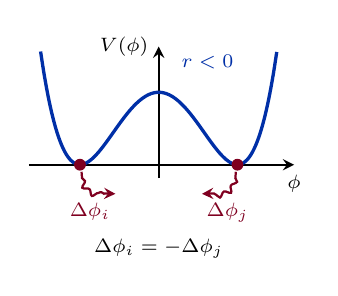
\begin{tikzpicture}[font=\scriptsize,>=stealth]
        \draw[->,thick] (-1.65,0.25) -- (1.72,0.25) node[below] {$\phi$};
        \draw[->,thick] (0,0.08) -- (0,1.75) node[left] {$V(\phi)$};
        \draw[very thick,Kleinblue,domain=-1.5:1.5,samples=80,smooth]
          plot (\x,{0.25+0.92*(\x*\x-1)^2});
        \node[Kleinblue] at (0.62,1.55) {$r<0$};
        \fill[burgundy] (-1,0.25) circle (0.075);
        \fill[burgundy] (1,0.25) circle (0.075);
        \draw[->,burgundy,thick,decorate,
              decoration={snake,amplitude=0.3mm,segment length=1.4mm,
                          pre length=0.8mm,post length=1.5mm}]
          (-0.98,0.16) .. controls (-0.98,-0.08) and (-0.84,-0.12) .. (-0.55,-0.12)
          node[midway,below=1pt] {$\Delta\phi_i$};
        \draw[->,burgundy,thick,decorate,
              decoration={snake,amplitude=0.3mm,segment length=1.4mm,
                          pre length=0.8mm,post length=1.5mm}]
          (0.98,0.16) .. controls (0.98,-0.08) and (0.84,-0.12) .. (0.55,-0.12)
          node[midway,below=1pt] {$\Delta\phi_j$};
        \node at (0,-0.82) {$\Delta\phi_i=-\Delta\phi_j$};
      \end{tikzpicture}
    \end{column}
  \end{columns}
  % align 在 minipage 末尾会丢掉 belowdisplayskip，没有这行下一栏会压到公式
  \vspace{2em}
  \begin{columns}[T,onlytextwidth]
    \begin{column}{0.44\textwidth}
      \centering
      Conserved mean\\[0.4em]
      $M(t)\equiv V^{-1}\!\int d^dx\,\phi(\bm{x},t)$\\[0.3em]
      $M(t)=M(0)$
    \end{column}
    \begin{column}{0.28\textwidth}
      \centering
      Critical dynamics\\[0.5em]
      $\tau\propto \xi^z$\\[0.2em]
      $\tau\propto k^{-z}$\\[0.2em]
      $z=4-\eta$
    \end{column}
    \begin{column}{0.22\textwidth}
      \centering
      Training pairs\\[0.5em]
      $\Delta t=10$
    \end{column}
  \end{columns}
  \vspace{0.4em}
  \begin{center}
    \scriptsize
    Hohenberg and Halperin, Rev. Mod. Phys. 49, 435 (1977).
  \end{center}
\end{frame}

% ---------------------------------------------------------------- 4
\begin{frame}{Equilibrium and nonequilibrium evolution}
  \begin{columns}
    \begin{column}{0.30\textwidth}
      {\bfseries\color{Kleinblue} Strongly coupled\\ critical point}\\
      $\kappa=0.34034$, $\lambda=1$\\
      $L=32$, $\Delta t=10$

      \vspace{0.2em}
      {\bfseries\color{Kleinblue} Initial ensembles}\\
      HMC equilibrium\\
      Gaussian quench

      \vspace{0.2em}
      {\bfseries\color{Kleinblue} Rollout}\\
      \alert{$\bm{200}$} kernel steps\\
      $t=2000$

      \vspace{0.2em}
      {\bfseries\color{Kleinblue} Checks vs SOSRA}\\
      $G_1(t)$ agrees\\
      $M(t)=M(0)$
    \end{column}
    \begin{column}{0.68\textwidth}
        \phantom{1em}
      \centering
      \includegraphics[width=0.9\linewidth]{validation_L32}
    \end{column}
  \end{columns}
\end{frame}

% ---------------------------------------------------------------- 5
\begin{frame}{The critical exponent emerges}
  \begin{columns}
    \begin{column}{0.44\textwidth}
      {\bfseries\color{Kleinblue} Normalized mode correlation}
      \small
      \begin{equation*}
        G_n(t)=V^{-1}\left\langle|\phi(\bm{k}_n,t)|^2\right\rangle
      \end{equation*}
      \begin{equation*}
        \rho_n(\Delta t)=
        \frac{\left\langle\operatorname{Re}\!\left[
          \phi(\bm{k}_n,t+\Delta t)\phi(\bm{k}_n,t)^*
        \right]\right\rangle_t}
        {\sqrt{
          \left\langle G_n(t+\Delta t)\right\rangle_t
          \left\langle G_n(t)\right\rangle_t}}
      \end{equation*}

      
      {\bfseries\color{Kleinblue} Dynamic scaling}
      \begin{equation*}
        \rho_n(\Delta t)=f(x),\qquad x=\frac{\Delta t}{\tau_n},
      \end{equation*}
      \begin{equation*}
        \tau_n\propto\widehat k_n^{-z},\quad
        \widehat k_n=\sqrt{8}\sin\!\frac{\pi n}{L}.
      \end{equation*}

      {\bfseries\color{Kleinblue} Fits at $L=32$}

      \alert{$\bm{z_{\rm DM}=3.792(19)}$}

      \alert{$\bm{z_{\rm SOSRA}=3.764(36)}$}
    \end{column}
    \begin{column}{0.54\textwidth}
      \includegraphics[width=\linewidth]{collapse_dm_L32}
        \scriptsize
      \textcolor{Kleinblue}{$z=4-\eta=15/4=3.75$}. \textcolor{burgundy}{\textbf{Exact.}} Halperin et al., PRB 10, 139 (1974).\\

      \textcolor{Kleinblue}{$z=3.83(10),\ 3.716(17)$}. \textcolor{burgundy}{\textbf{MC.}} Schweitzer et al., NPB 984, 115944 (2022).\\

      \textcolor{Kleinblue}{$z=3.95(10)$}. \textcolor{burgundy}{\textbf{Kawasaki MC.}} Zheng, PLA 277, 257 (2000), erratum 282, 132 (2001).\\

      \textcolor{Kleinblue}{$z=3.79\pm0.05$}. \textcolor{burgundy}{\textbf{MC RG.}} Moseley et al., J. Stat. Phys. 57, 421 (1989).\\

      \textcolor{Kleinblue}{$z=3.80$}. \textcolor{burgundy}{\textbf{MC RG.}} Yalabik and Gunton, PRB 25, 534 (1982).
    \end{column}
  \end{columns}
\end{frame}

% ---------------------------------------------------------------- 6
\begin{frame}{Prediction on unseen $L=64$}
  \begin{columns}
    \begin{column}{0.44\textwidth}
      {\bfseries\color{Kleinblue} Size extrapolation}

      \small
      \begin{center}
        $L_{\rm train}=8,16,32$\ \ {$\Longrightarrow$}\ \ \alert{$\bm{L=64}$}\\[0.4em]
        32 network calls
      \end{center}

      {\bfseries\color{Kleinblue} Fits at $L=64$}

      \alert{$\bm{z_{\rm DM}=3.855(21)}$}

      \alert{$\bm{z_{\rm Model\,B}=3.867(23)}$}

      \vspace{0.6em}
      {\bfseries\color{Kleinblue} As fast as the best direct solver}

      \scriptsize
      512 trajectories, $t=100$, GH200, matched accuracy
    \end{column}
    \begin{column}{0.54\textwidth}
      \centering
      \includegraphics[width=\linewidth,height=0.40\textheight,keepaspectratio]{reverse_nfe_tau_L64}
      \par\vspace{0.4em}
      {\raggedright
        \scriptsize
        \setlength{\tabcolsep}{2pt}
        \begin{tabular}{lcc}
          \toprule
          & \multicolumn{2}{c}{Wall time (s)} \\
          \cmidrule(lr){2-3}
          Method & equil. & noneq. \\
          \midrule
          \alert{DPM-Solver-v3 (This work)} & $3.24$ & $3.26$ \\
          SOSRA (This work) & $1.30$ & $3.28$ \\
          SOSRA (StochasticDiffEq.jl) & $12.36$ & $30.67$ \\
          ShARK (Diffrax) & $5.56$ & $17.76$ \\
          EM (Diffrax) & $19.45$ & $38.75$ \\
          EM (other GPU/CPU solvers) & $>100$ & $>200$ \\
          \bottomrule
        \end{tabular}
      \par}
    \end{column}
  \end{columns}
\end{frame}

% ---------------------------------------------------------------- 7
\begin{frame}{Phase separation on unseen $L=128$}
  \begin{columns}[T]
    \begin{column}{0.44\textwidth}
      {\bfseries\color{Kleinblue} Sign-field correlation}
      \small
      \begin{equation*}
        \sigma(\bm{x},t)=\operatorname{sgn}\phi(\bm{x},t)
      \end{equation*}
      \begin{equation*}
        C(r,t)=\left\langle\sigma(\bm{x},t)\,\sigma(\bm{x}+\bm{r},t)\right\rangle
      \end{equation*}

      $L(t)$: first zero of $C(r,t)$

      {\bfseries\color{Kleinblue} Phase-ordering scaling}
      \begin{equation*}
        C(r,t)=g\big(r/L(t)\big)
      \end{equation*}
      \begin{equation*}
        L(t)\propto t^{1/3}
      \end{equation*}

      {\bfseries\color{Kleinblue} Size extrapolation}

      $L_{\rm train}\le64$\ \ {$\Longrightarrow$}\ \ \alert{$\bm{L=128}$}

      \alert{$\bm{L(t)\propto t^{1/3}}$}\\[0.2em]
      $L_{\rm DM}/L_{\rm SOSRA}=1$ within $2\%$
    \end{column}
    \begin{column}{0.54\textwidth}
      \centering
      \vspace*{-0.6em}
      \includegraphics[width=\linewidth,height=0.58\textheight,keepaspectratio]{collapse_dm_L128}
      \par\vspace{0.15em}
      {\raggedright
      \fontsize{5.2}{5.2}\selectfont
      \textcolor{Kleinblue}{$t^{1/3}$}. \textcolor{burgundy}{\textbf{LSW theory.}} Lifshitz and Slyozov, JPCS 19, 35 (1961).\\
      \textcolor{Kleinblue}{Asymptotic $t^{1/3}$, corrections}. \textcolor{burgundy}{\textbf{Conserved Ising.}} Huse, PRB 34, 7845 (1986).\\
      \textcolor{Kleinblue}{$t^{1/3}$, scaling}. \textcolor{burgundy}{\textbf{2D critical Model B.}} Rogers et al., PRB 37, 9638 (1988).\\
      \textcolor{Kleinblue}{$t^{1/3}$ scaling}. \textcolor{burgundy}{\textbf{Review.}} Bray, Adv. Phys. 43, 357 (1994).\\
      \textcolor{Kleinblue}{$t^{1/3}$}. \textcolor{burgundy}{\textbf{Polymer experiment.}} Krausch et al., PRL 71, 3669 (1993).\\
      \textcolor{Kleinblue}{Critical $\alpha=1/3$}. \textcolor{burgundy}{\textbf{2D CH.}} K\"onig et al., PCCP 23, 24823 (2021).\\
      \textcolor{Kleinblue}{$\alpha_L=0.34,0.37$ from perimeter}. \textcolor{burgundy}{\textbf{Membrane.}} Zhiliakov et al., BBA 1863, 183446 (2021).\\
      \textcolor{Kleinblue}{$t^{1/3}$}. \textcolor{burgundy}{\textbf{Passive membrane, CH.}} Arnold et al., PRL 131, 128402 (2023).\\
      \textcolor{Kleinblue}{$t^{1/3}$}. \textcolor{burgundy}{\textbf{HP1 Model B.}} Tortora et al., PNAS 120, e2211855120 (2023).\\
      \textcolor{Kleinblue}{Long-time $t^{1/3}$}. \textcolor{burgundy}{\textbf{Diffusive polymer Model B.}} Garcia et al., JCP 159, 214904 (2023).
      \par}
    \end{column}
  \end{columns}
\end{frame}

% ---------------------------------------------------------------- 8
\begin{frame}{Summary}
  \begin{center}
    {\large Paired snapshots $\longrightarrow$ long-time stochastic dynamics}
  \end{center}
  \vspace{1.2em}
  \begin{columns}[T,onlytextwidth]
    \begin{column}{0.31\textwidth}
      \centering
      {\small Critical relaxation}\\[0.8em]
      {\alert{\large $z_{\rm DM}=3.792$}}\\[0.4em]
      {\small $z_{\rm SOSRA}=3.764$}
    \end{column}
    \begin{column}{0.31\textwidth}
      \centering
      {\small Beyond training sizes}\\[0.8em]
      {$L_{\rm train}\le64$}\\[0.4em]
      {\alert{\Large $L=128$}}
    \end{column}
    \begin{column}{0.31\textwidth}
      \centering
      {\small Phase separation}\\[0.8em]
      {\alert{\large $L(t)\propto t^{1/3}$}}\\[0.4em]
      {\small within $2\%$}
    \end{column}
  \end{columns}
  \vfill
  \begin{center}
    {\large Thank you!}
  \end{center}
\end{frame}

\end{document}
